\documentclass[a4paper]{article}
\usepackage[T1]{fontenc}
\usepackage[utf8]{inputenc}
\usepackage{fancyhdr}
\usepackage{vmargin}
\usepackage{multirow}	
\usepackage{amsmath}
\usepackage{amssymb}
\usepackage{comment}
\usepackage{url}
\usepackage{graphics}
\usepackage{graphicx}
\usepackage{grffile}
\usepackage{color}
\usepackage{framed}
\usepackage{hyperref}
\usepackage{epsfig}
\usepackage{tikz}
\usepackage{float}
\usepackage{subcaption}
\usepackage{forest,calc}
\usepackage{tikz-qtree}
\usepackage{color}
\usepackage{colortbl}
\usepackage{capt-of}

\setlength{\parindent}{0pt}
\setlength{\parskip}{5pt}
\setlength{\headheight}{24pt}
\setlength{\headsep}{24pt}

\frenchspacing
\pagestyle{fancy}
\sloppy

\markright{headline}

% Kopfzeile
\lhead{\begin{tabular}{l}
\textbf{Software Project}  \\
\subtitle \\
\end{tabular}}

\rhead{\begin{tabular}{rc} 
\StudNameOne\\
\StudNameTwo\\
\StudNameThree\\
\StudNameFour\\
\end{tabular}}

\author{\StudNumeOne}

\newcommand{\subtitle}{\textbf{Singing Voice Synthesis with DiffSinger}}
\newcommand{\StudNameOne}{\textbf{David Matkovic} - 7038335 }
\newcommand{\StudNameTwo}{\textbf{Jona Hoppe} - 7034173}
\newcommand{\StudNameThree}{\textbf{Hanna Helbig} - 7008726}
\newcommand{\StudNameFour}{\textbf{Maximilian Schmidt} - 2356}

\usepackage{setspace}  % Include the setspace package

\onehalfspacing


\begin{document}

%==============================================
%================ Introduction =================
%==============================================
\section*{Introduction}


%==============================================
%================ Preprocessing ================
%==============================================
\section{Preprocessing}

\subsection{Initial Preprocessing}
The initial phase of our project focused on preprocessing the audio data, which is a crucial step that encompasses several subtasks. The preprocessing aims at preparing the raw material for further analysis.

\subsubsection{Data Acquisition}
The first step before we could start with the preprocessing involved acquiring the songs that we wanted to use for our project. We wanted to ensure a diverse and representative dataset; thus, we searched for publicly available audio collections of Linkin Park. As we did not find a complete collection, we sourced the audios from YouTube. In total, we curated a corpus consisting of eight albums, each containing an average of 12 tracks. This collection formed the foundation for our subsequent processing and analysis steps.

After collecting the data, we started with the preprocessing. Preprocessing is of critical importance for singing voice synthesis, especially when working with raw audio data, which is typically noisy and includes irrelevant or disturbing elements, such as instrumentals, audience noise, and silences, all of which can have a negative impact on model performance \cite{Kulkarni2023}.

As we wanted to train the model to recognize the specific patterns of Chester Bennington’s voice, including his pitch, timbre and vocal fry, a good preprocessing is important to ensure that all relevant information is captured by the model and all irrelevant information (noise, other voices, instrumentals) is excluded to provide the best learning. Including instrumentals and noisy data would potentially lead to the model learning these unwanted features, resulting in a bad overall model output. This being said, we tried to preprocess our data, such that we excluded instrumentals and noise and included clean singing voice data, which was later passed through the model.

<<<<<<< HEAD
\subsubsection{Segmentation}
After the vocal extraction, the next step was to segment the data. Segmenting the audios into smaller chunks is important as it can significantly enhance the model’s performance and the reliability of the forced alignment that followed this step \cite{Rybach2009}. The quality of the alignment heavily depends on the segmentation, as a wrong segmentation will lead to a wrong alignment. The effectiveness of our model is, therefore, closely tied to the goodness of the audio segmentation. 
=======
\subsubsection*{Segmentation}
After the vocal extraction, the next step was to segment the data. Segmenting the audios into smaller chunks is important as it can significantly enhance the model’s performance and the reliability of the forced alignment that followed this step \cite{Rybach2009}. The quality of the alignment heavily depends on the segmentation, as a wrong segmentation will lead to a wrong alignment. The effectiveness of our model is, therefore, closely tied to the goodness of the audio segmentation.
>>>>>>> 7ef8c5b9b17717688e8230bc0116750a54caace7

The best way to ensure a good segmentation would be to do it manually, however, as our dataset is quite big, this would have been out of the scope of this project, so we searched for automatic segmentation methods.

We tried different methods for automatic segmentation. We first used pydub, which is a Python library and a known powerful tool for preprocessing audio and text data, widely utilized in speech and text recognition applications \cite{Kulkarni2023}. We also tried pydub.silence, which is a module in the Python pydub library that provides functions to detect and handle silent segments in audio files. After that, we used Whisper, which is a powerful automatic speech recognition system developed by OpenAI \cite{OpenAI2022}. Whisper is trained on 680,000 hours of diverse, multilingual, and multitask data from the web, which makes it a robust model that can handle accents, background noise, and technical or domain-specific language, making it a suitable choice for our project, as speech clarity and variability are some of our main challenges. Whisper supports transcriptions for multiple languages. During the description, Whisper detects voice activity and attenuates background noise or music. In order for Whisper to work, PyTorch and ffmpeg must also be installed (those are its dependencies) \cite{Andreyev2025}. Whisper is not intended for real-time transcription and is designed to process audio containing at least one complete sentence, ideally under 30 seconds in length.

Whisper's main challenge lies in balancing accuracy and resource efficiency, as it can produce hallucinated transcriptions and larger models demand high computational power, which limits their usability on resource-constrained devices \cite{Andreyev2025}.

We also used whisper-timestamped, which is an extension of whisper and provides more efficient and accurate word timestamps. Whisper-timestamped uses a Dynamic Time Warping approach, which allows it to create word timestamps and a more accurate estimation on speech segments. As a result, the estimated start and end times of speech segments are more precise. Another advantage over the base model is that Whisper Timestamped can process longer files \cite{Andreyev2025}.

Whisper-timestamped turned out to be the best model to segment our audios. It works with different model sizes: base, small, medium, and large. We used the small model as it was sufficiently well.

Following an initial phase of trial and error, we implemented a custom script utilizing whisper-timestamped to segment our audio data. The script first verifies the file format, ensuring that only audio files (with the ending wav or mp3) are processed and that only those files whose names conformed to our naming convention (i.e., filenames containing either six or nine digits) were included. Once the appropriate files were selected, we used whisper-timestamped to generate segment-level transcriptions along with time-aligned boundaries. Most of the segments were fine, but some segments were extremely short (i.e., less than two seconds). To avoid these short segments and to enhance the usability of the resulting segments for annotation purposes, we introduced a minimum segment duration of four seconds. Thus, segments falling below this threshold were automatically concatenated with the subsequent segment to ensure that each snippet was sufficiently long to carry meaningful context for the automatic labeling. We also had some issues with hard cuts, where word endings were cut off too strictly. To mitigate this problem, we introduced a small buffer between consecutive segments (0.1s). This slight overlap helped preserve the natural flow of speech and ensured smoother transitions, which improved both the accuracy of our transcriptions and the overall quality of the audio snippets.

<<<<<<< HEAD
\subsubsection{Manual Segmentation}
=======
After segmenting our data, we had to align our audio data with textual/phonetic annotations. Here, we encountered another challenge as some segments were silent, resulting in an error, thus, we excluded segments with zero variance before aligning the data.

\subsubsection*{Alignment Tools}
We initially used the Montreal Forced Aligner (MFA), which is a widely recognized tool for automatic speech-text alignment. The MFA is built upon the Kaldi speech recognition toolkit. It is designed to provide robust phonetic segmentation by leveraging triphone acoustic models and speaker adaptation techniques \cite{McAuliffe2017}. MFA has been successfully applied to various languages and datasets; however, in our case, the MFA did not reveal convincing results. We attributed this to the fact that the MFA is primarily designed for spoken language, while singing poses some additional challenges, such as extended phonemes and pitch variations.

To improve alignment quality, we explored alternative tools and came across SOFA (Singing-Oriented Forced Aligner), which functions similarly to the Montreal Forced Aligner (MFA) but is specifically designed for singing voice. According to its Github page, SOFA offers simpler installation, better performance, and faster inference speed compared to MFA. After testing it on a few examples, we observed slightly improved results \cite{Greenleaf2001}; however, the alignments were still not consistently convincing. We continued our search and discovered LabelMakr, “a GUI tool to help users easily generate SVS phoneme-level labels” \cite{spicytigermeat} for singing voice synthesis (SVS), particularly intended for use with DiffSinger. While initial tests with a small sample also fell short of expectations, we observed that LabelMakr's performance significantly improved when it was applied to our full dataset, such that we ended up with some meaningful alignments that we used for our training.

\subsubsection*{Data Conversion with nnsvs-db-converter}
We used the nnsvs-db-converter, a Python tool for converting vocal databases with HTS mono labels into DiffSinger format to make them compatible with variance models for predicting pitch and timing \cite{nnsvsdbconverter}. It handles sample segmentation by ensuring that each sample has a maximum length and an acceptable number of pauses between segments, and converts silent phonemes (e.g., sil, pau) to standardized representations (SP and AP for breaths). The script requires minimal external dependencies, making it easily accessible. In addition, it supports language definitions that specify vowels and liquids for better segmentation and timing handling, and it can estimate MIDI pitch and timing information for the use of variance models.

In our project, we used this converter to convert our .lab files, which contained the phoneme alignments, into .ds files to ensure they were compatible with the DiffSinger framework and could utilize variance-based pitch and timing predictions.

\subsubsection*{SlurCutter Exploration}
We also had a look into SlurCutter, which is a specialized tool that is designed to assist in the creation of datasets for DiffSinger. Its primary function is to edit MIDI sequences that are stored in .ds files to facilitate the preparation of data for variance model training \cite{openvpi}. However, it requires a lot of time and effort as this process is done manually, so we decided not to do it on a large scale.

\subsubsection*{Manual Segmentation}
>>>>>>> 7ef8c5b9b17717688e8230bc0116750a54caace7
To include more data and improve model performance, we additionally included two live albums in our dataset. As many segments contained screaming from the audience, we went through them and cut out unwanted parts manually with Praat, a tool for speech analysis and phonetic research.


\begin{figure}[htbp]
    \centering
    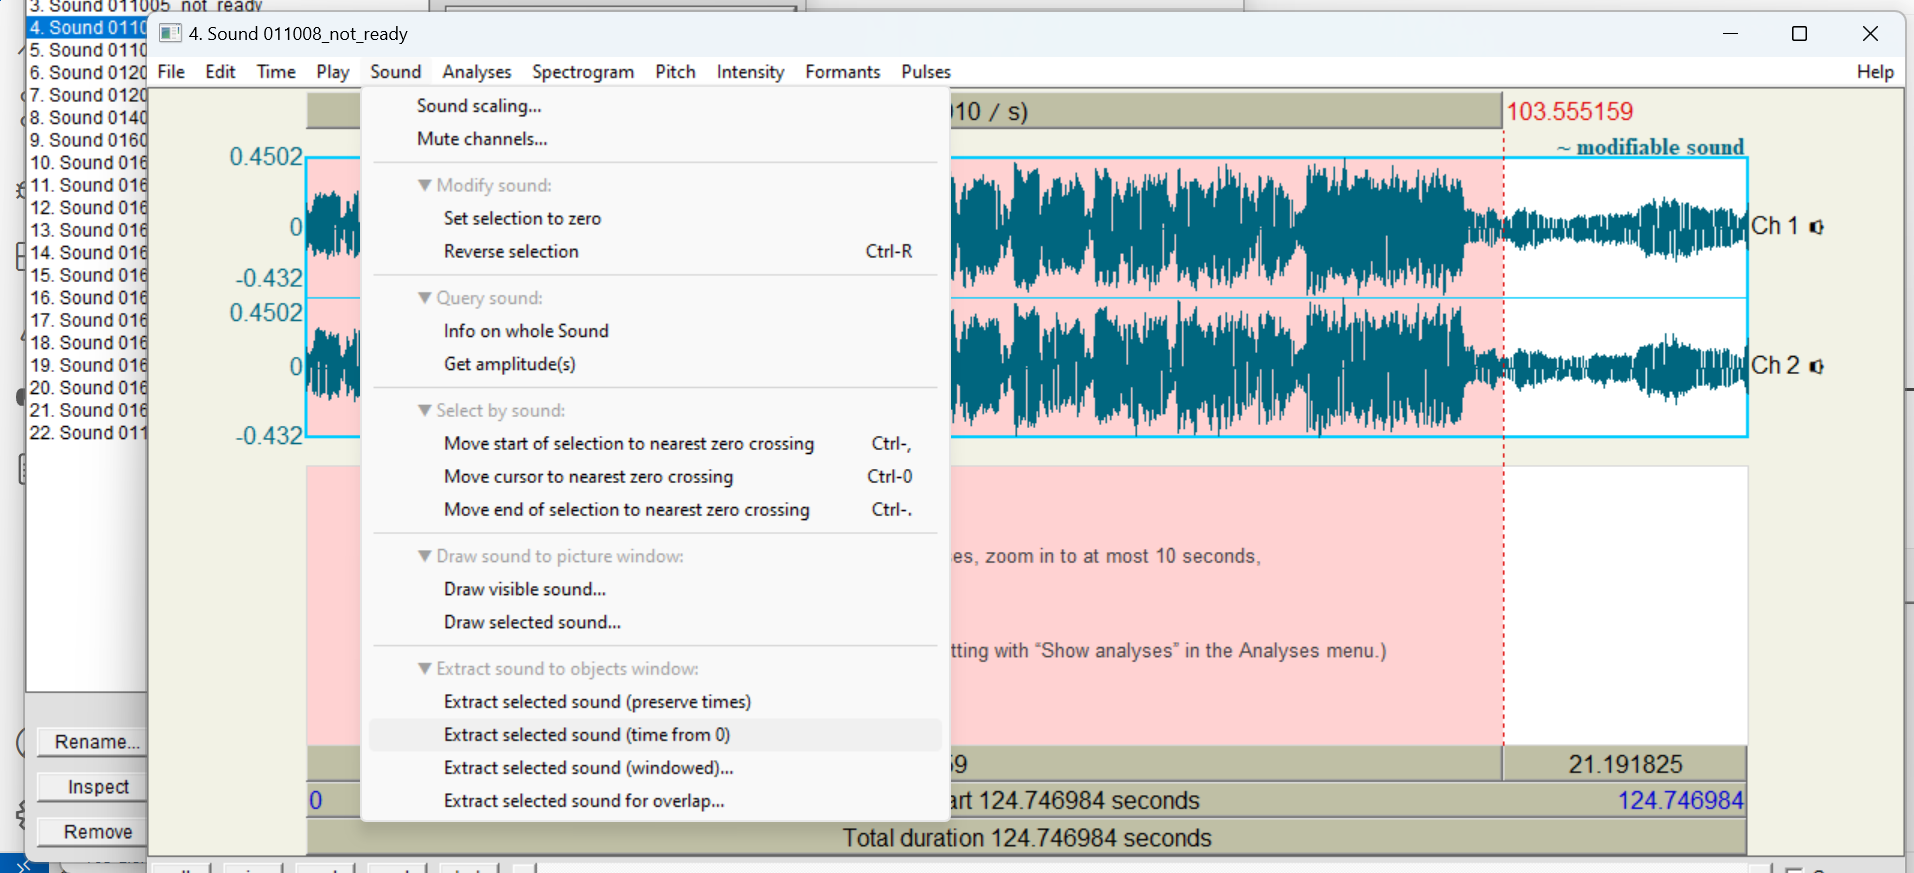
\includegraphics[width=0.5\textwidth]{graphics/cutting_noise.png}
    \caption{excluding noisy screams at the end of the audio snippet}
    \label{fig:bild1}
\end{figure}

After segmenting our data, we had to align our audio data with textual/phonetic annotations. Here, we encountered another challenge as some segments were silent, resulting in an error, thus, we excluded segments with zero variance before aligning the data.

\subsubsection{Alignment Tools}
We initially used the Montreal Forced Aligner (MFA), which is a widely recognized tool for automatic speech-text alignment. The MFA is built upon the Kaldi speech recognition toolkit. It is designed to provide robust phonetic segmentation by leveraging triphone acoustic models and speaker adaptation techniques \cite{McAuliffe2017}. MFA has been successfully applied to various languages and datasets; however, in our case, the MFA did not reveal convincing results. We attributed this to the fact that the MFA is primarily designed for spoken language, while singing poses some additional challenges, such as extended phonemes and pitch variations. 

To improve alignment quality, we explored alternative tools and came across SOFA (Singing-Oriented Forced Aligner), which functions similarly to the Montreal Forced Aligner (MFA) but is specifically designed for singing voice. According to its Github page, SOFA offers simpler installation, better performance, and faster inference speed compared to MFA. After testing it on a few examples, we observed slightly improved results \cite{Greenleaf2001}; however, the alignments were still not consistently convincing. We continued our search and discovered LabelMakr, “a GUI tool to help users easily generate SVS phoneme-level labels” \cite{spicytigermeat} for singing voice synthesis (SVS), particularly intended for use with DiffSinger. While initial tests with a small sample also fell short of expectations, we observed that LabelMakr's performance significantly improved when it was applied to our full dataset, such that we ended up with some meaningful alignments that we used for our training.

\subsubsection{Manual Alignment}
In addition to our segmented audio snippets, we fully labeled two complete songs — Over Each Other and The Emptiness Machine — using LabelMakr, which we later used during inference. Since these full-song annotations were created after the short segments had already been labeled, the initial alignments were expectedly poor. To address this, we manually refined the boundaries: we shifted misaligned ones, added missing boundaries, and removed others — particularly SP (speech pause) and AP (aspiration pause) annotations, which frequently appeared in inappropriate positions.

\begin{figure}[htbp]
    \centering
    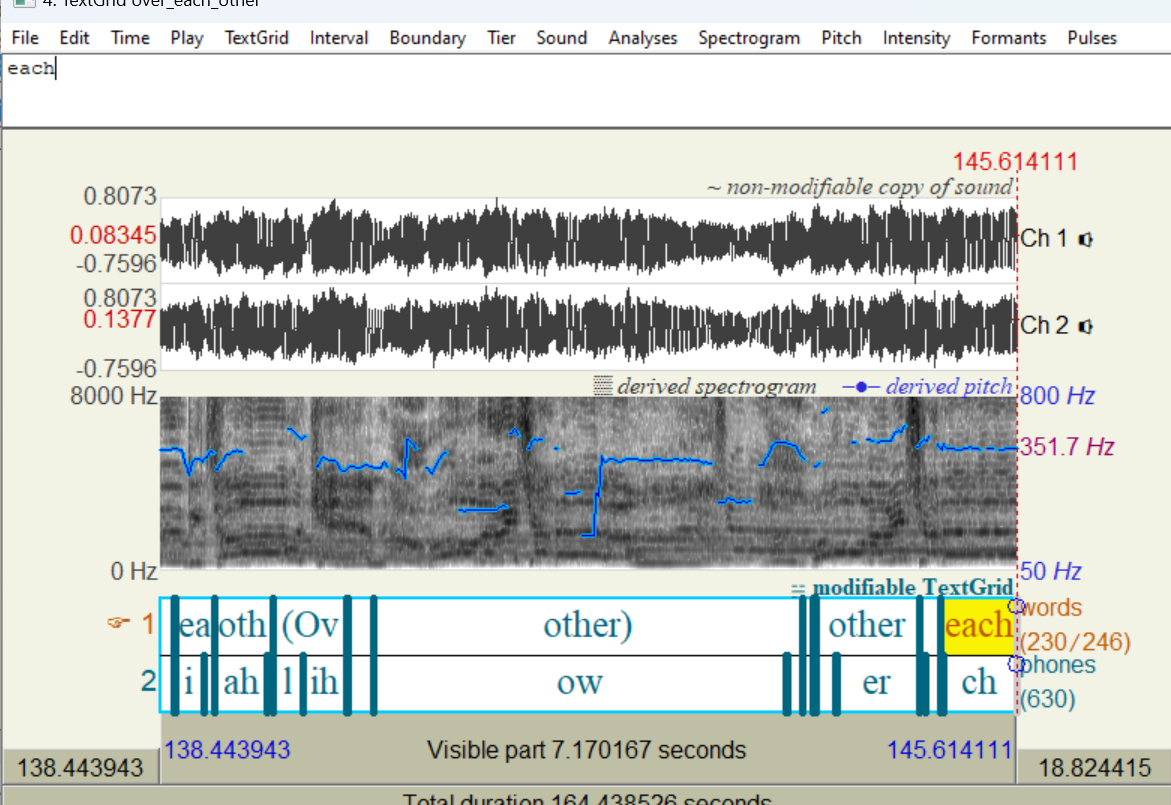
\includegraphics[width=0.5\textwidth]{graphics/bad_alignment.png}
    \caption{bad alignment}
    \label{fig:bild2}
\end{figure}

\begin{figure}[htbp]
    \centering
    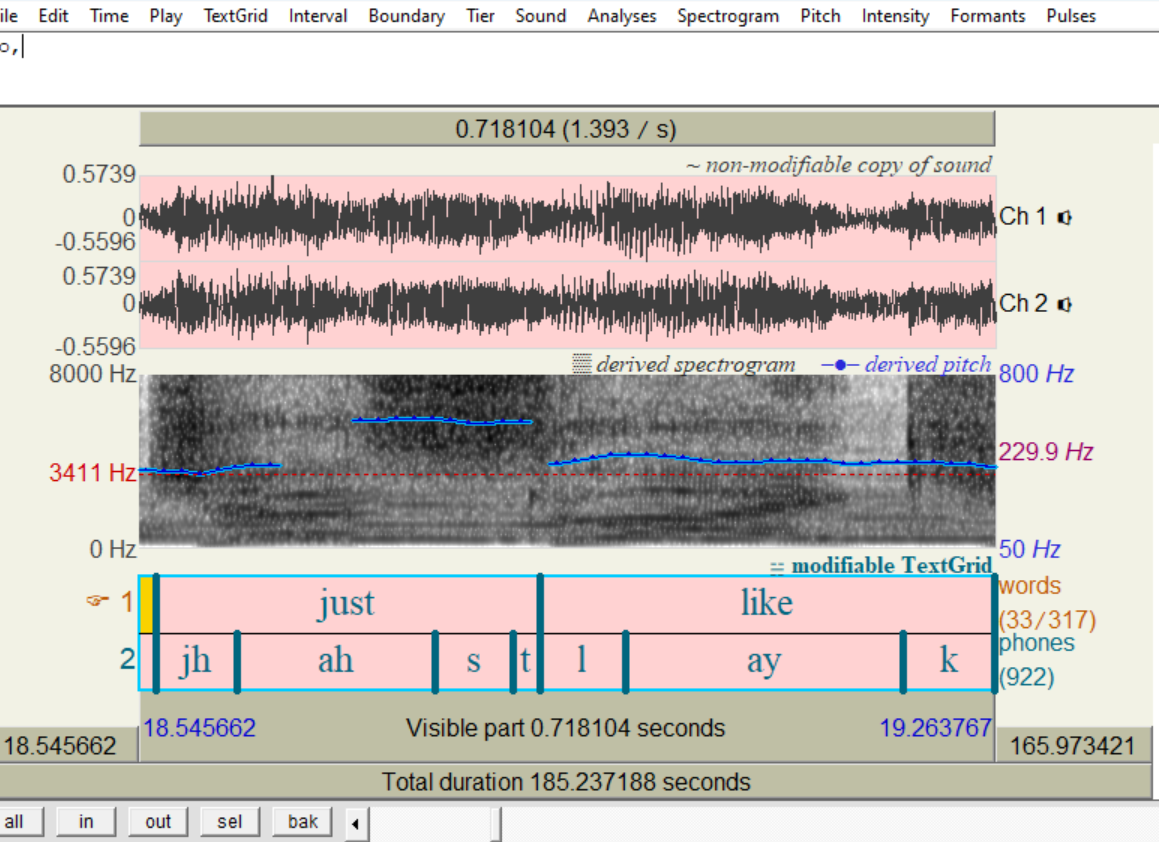
\includegraphics[width=0.5\textwidth]{graphics/manual_alignment.png}
    \caption{manual alignment}
    \label{fig:bild3}
\end{figure}

\subsubsection{Data Conversion with nnsvs-db-converter}
We used the nnsvs-db-converter, a Python tool for converting vocal databases with HTS mono labels into DiffSinger format to make them compatible with variance models for predicting pitch and timing \cite{nnsvsdbconverter}. It handles sample segmentation by ensuring that each sample has a maximum length and an acceptable number of pauses between segments, and converts silent phonemes (e.g., sil, pau) to standardized representations (SP and AP for breaths). The script requires minimal external dependencies, making it easily accessible. In addition, it supports language definitions that specify vowels and liquids for better segmentation and timing handling, and it can estimate MIDI pitch and timing information for the use of variance models.

In our project, we used this converter to convert our .lab files, which contained the phoneme alignments, into .ds files to ensure they were compatible with the DiffSinger framework and could utilize variance-based pitch and timing predictions.

\subsubsection{SlurCutter Exploration}
We also had a look into SlurCutter, which is a specialized tool that is designed to assist in the creation of datasets for DiffSinger. Its primary function is to edit MIDI sequences that are stored in .ds files to facilitate the preparation of data for variance model training \cite{openvpi}. However, it requires a lot of time and effort as this process is done manually, so we decided not to do it on a large scale.



\subsection{Refined Preprocessing}
As our initial training revealed noisy outputs, we decided to improve our dataset to enhance model performance. We began by manually manipulating two albums, where we removed segments that contained excessive noise, overlapping voices, or rap sections. The result was a cleaned subset of data, which we stored as our clear training data.

To scale this cleaning process across the entire dataset, we wrote several scripts to automate the filtering process. First, we analyzed how different types of data snippets varied across the corpus. We manually selected representative examples of each category—screaming, multi-voice, clear voice, and rap—and stored them in separate folders to serve as our reference data.

Initially, we attempted to map each song snippet to the category it was most similar to. However, this yielded inconsistent and often unreliable classifications, such that the categories had a large overlap and seemed to be meaningless. We then tried to identify dominant acoustic features that could meaningfully distinguish between categories. We found that fundamental frequency was a strong discriminator between screaming and clear singing. After analyzing our reference examples, we set a threshold of 230 Hz to filter out heavy screams and background noise—this removed many problematic segments while retaining the majority of clean vocals. The remaining screams in the clean voice examples were retained as they were less problematic than the really heavy ones and the background noises.

To distinguish between rap and singing, we found that syllable rate is a suitable discriminator. Since our target singer, Chester Bennington, does not perform the rap sections, we applied a threshold of six syllables per second to exclude the fast-paced vocal segments.

For segments with multiple overlapping voices, we explored various characteristics and thresholds, but none of them seemed to be a reliable discriminator. Therefore, we returned to the similarity-based approach—this time using only a single, well-chosen example per category to guide the classification, which surprisingly seemed to work better than with the bigger example set. While the categories were still imperfect, this method provided the most usable approximation.

Ultimately, we combined the resulting clear voice set (without screams, rap, multiple voices) with other data to train three of our models (see model training).






%==============================================
%================ Training =====================
%==============================================
\section{Training}

\subsection{Manual Augmentation}

Data augmentation plays a crucial role in improving the fine-tuning and accuracy of speech attributes like pitch, loudness, and duration, enhancing the quality of AI-generated singing \cite{Morrison2024}.
To enhance the diversity and robustness of our audio dataset, we implemented several data augmentation techniques: pitch shifting, loudness adjustment, noise reduction, and speed alteration. These methods are widely recognized for their effectiveness in improving speech recognition models by simulating speaker variations \cite{Morrison2024}. As singing is especially prone to these elements (e.g., pitch, loudness, and speed change drastically during a song), these augmentation techniques appeared to be especially useful for our purposes.

\begin{itemize}
    \item \textbf{Pitch Shifting}: We wrote a script to adjust the pitch of each audio file by a semitone both upwards and downwards, creating two additional variations per original file. This technique helps the model become invariant to pitch differences as the pitch changes heavily between Chester’s different singing modes (e.g., compare harmonic singing versus screaming). We also tried to make more drastic pitch shifting, however, then the voice seemed to be too different from the original, so we did not include it in our model training.

    \item \textbf{Loudness Adjustment}: The audio files’ loudness was modified by increasing and decreasing the volume by 10\%. This approach aids the model in handling variations in speaking volume and recording conditions.

    \item \textbf{Noise Reduction}: We applied a noise reduction technique to suppress background noises such as ambient sounds and audience noise. This process aimed to enhance the clarity of the singing voice and thus, enhance model performance. However, we found that the denoising also suppressed the screaming parts quite a bit, so we decreased the initially high penalty to only 30\% noise reduction and used a less strict high-pass filter. For some parts, the screaming was still denoised too heavily, however, we used the denoised parts too to make the model more robust.

    \item \textbf{Speed Alteration}: The speed of the audio recordings was adjusted by $\pm$10\%, creating versions that are slightly faster and slower than the original. This method exposes the model to variations in singing rates, improving its ability to generalize across different singing tempos.
\end{itemize}

By incorporating these augmentation strategies, we aimed to increase the robustness of the model, leading to better overall performance.


\subsubsection{Model 7 (manual + sorted clean)}

\begin{figure}[htbp]
    \centering
    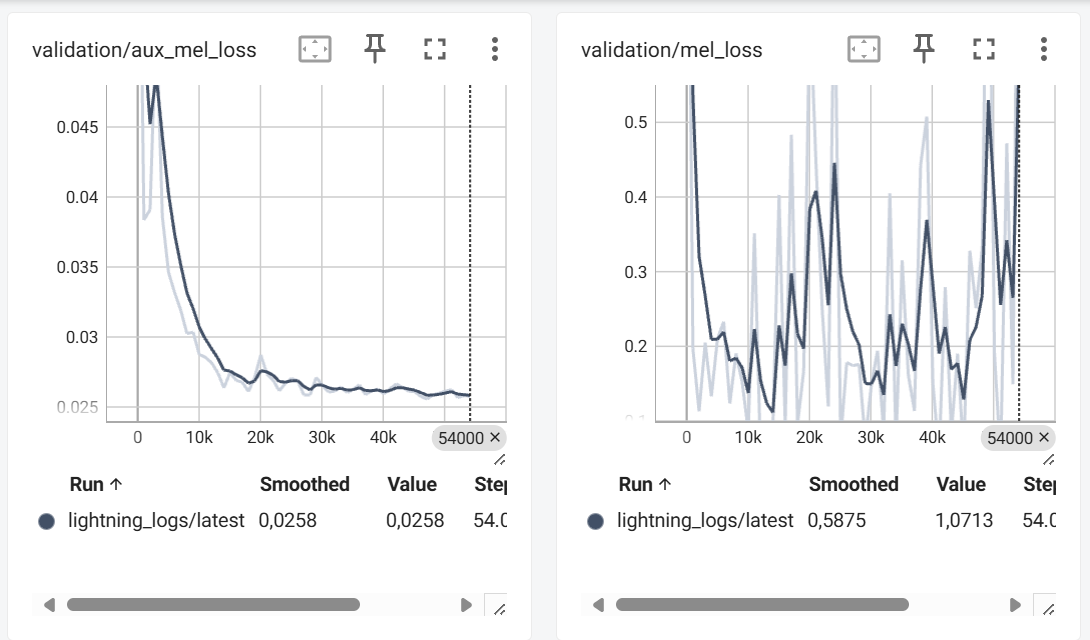
\includegraphics[width=0.5\textwidth]{graphics/v7_testing.png}
    \caption{model 7}
    \label{fig:bild4}
\end{figure}

As the dataset of the clean model seemed to be too small, we aimed to increase it. However, we wanted to include only “good” audio snippets, therefore, we used some scripts to automatically select other snippets that were considered to be “clean” (see refined preprocessing). This increased the dataset size to more than double the instances compared to the clean model. For this model, we used a batch size of 64 and 8 validation samples. The learning rate was set to 0.006. The model was trained for 54k epochs until the validation loss reached 0.026.

\subsubsection{Model 8 (manual + sorted + augmented clean)}

\begin{figure}[htbp]
    \centering
    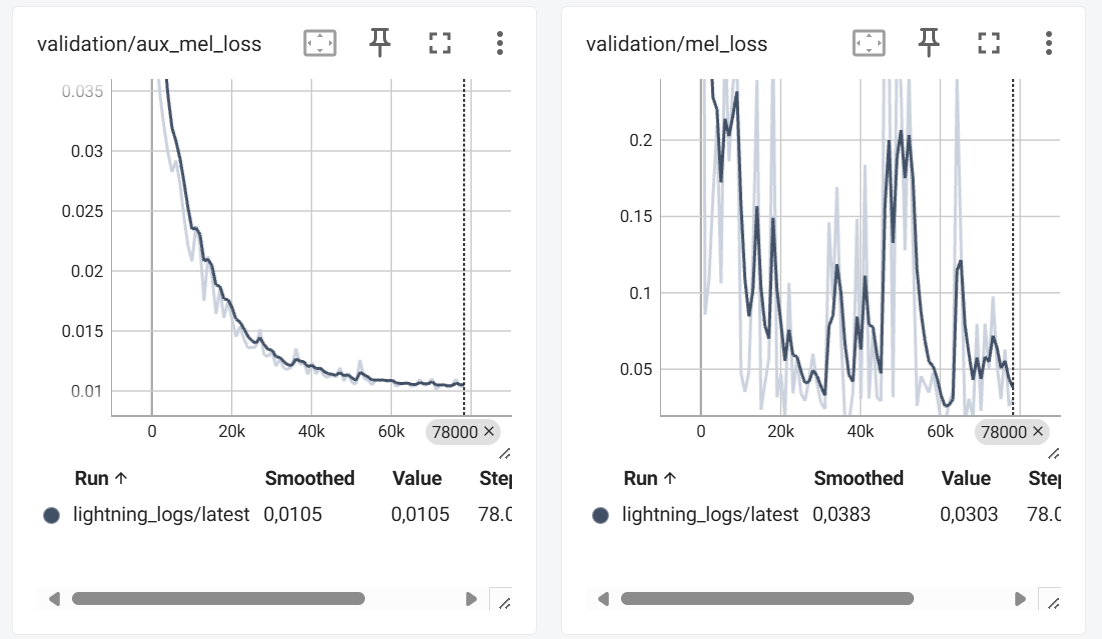
\includegraphics[width=0.5\textwidth]{graphics/v8_testing.png}
    \caption{model 8}
    \label{fig:bild5}
\end{figure}

As we still wanted to further augment our dataset, we trained the next model with an augmented dataset. We used the segments that we manually selected and those that were selected by the scripts and used different data augmentation techniques, such as pitch shifting, time shifting, noise reduction and loudness shifting (see data augmentation) to artificially enlarge our dataset. The batchsize was set to 64, eight validation samples were used and the learning rate was kept at 0.006. The model was trained for 78k epochs until the validation loss reached almost 0.01.


\subsubsection{Model 9 (large + augmented)}

\begin{figure}[htbp]
    \centering
    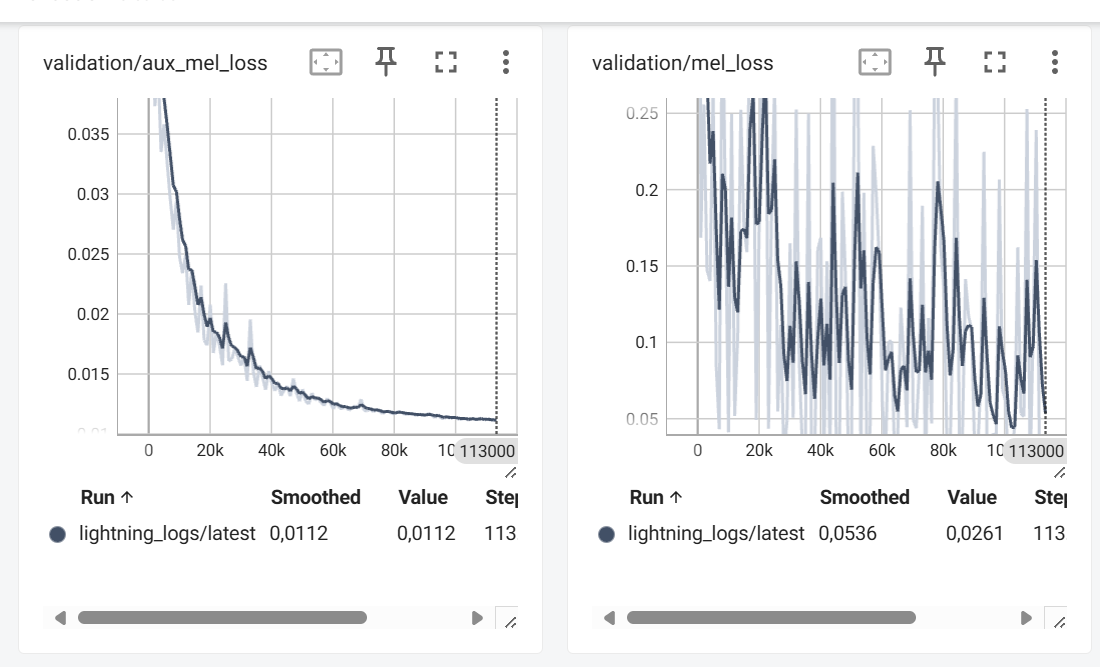
\includegraphics[width=0.5\textwidth]{graphics/v9_testing.png}
    \caption{model 9}
    \label{fig:bild5}
\end{figure}

Our last attempt was to train a model with data augmentation that included even more data (almost the entire dataset, except for some filtered noise/screams and rap), even though this data included some more overlapping singing and try data augmentation on this model as well. The parameters were kept constant compared to the smaller augmented model. However, this time we used our fine-tuned vocoder. We stopped the training after 113k epochs when it reached a validation loss of 0.011.


%==============================================
%================ Evaluation ===================
%==============================================
\section{Evaluation}

\subsection*{DiffSinger}
The base model we used for our training and synthesizing is DiffSinger. It is an
acoustic model, meaning it can map linguistik and symbolic input (like text or
notes) into acoustic features, used to generate actual audio. Acoustic features
include the most common feature mel-spectograms, but can also include linear
spectograms, F0 and pitch contour, and energy. It is also a variance model,
which is needed when trying to synthesize actual singing. A variance model
models the acoustic variations, for example pitch, energy and duration of sound.
The variance model predicts, based on the training data, how the voice features
should vary over time, based on the input. To avoid long computation time and
large resource needs, DiffSinger uses a shallow diffusion model. Traditional
diffusion models generate data, by starting with pure, random noise, and step by
step denoising it. This inference process is slow and takes many steps for just
a single generated sample. The shallow diffusion model used by DiffSinger is a
simpler and faster version of a full diffusion model. It uses fewer steps, but
often starts with a better starting point (for example a prediction from another
model). DiffSinger uses a non-diffusion model to predict a rough mel-spectogram
for the synthesized data, and refines it using the shallow diffusion model. By
using this technique, a lot of unnecessary steps, resources and computation time
are saved. Not using another model to make a first prediction would cause the
generated data to be a lot worse, since less steps are used and therefore less
noise is removed.

\subsection*{Choosing a model}

To be able to choose the best model for generating the vocals, we had to
evaluate them. We chose five different evaluation criteria. These criteria were
\emph{subjective Mean Opinion Score (MOS-LQS)}, \emph{comparison of histograms
    created from mel spectrograms}, \emph{objective Mean Opinion Score (MOS-LQO) as
    Perceptual Evaluation of Speech Quality (PESQ) score}, the \emph{root mean
    square error of F0 values (F0 RMSE)}, and the \emph{Speech-to-Noise ratio
    (SNR)}. \\
Each model was evaluated based on these criteria, and compared to the original
sound files. "gt" in the model lists refer to the \emph{ground truth}, or
original sound files. The other names refer to the respective model iteration.

\subsection*{Used files}
The following 14 segments were used in the evaluation:
\begin{itemize}
    \item Segment 22 from album 1, song 4
    \item Segment 3 from album 1, song 5
    \item Segment 1 from album 1, song 8
    \item Segment 22 from album 1, song 8
    \item Segment 5 from album 2, song 4
    \item Segment 7 from album 2, song 6
    \item Segment 17 from album 2, song 6
    \item Segment 1 from album 2, song 9
    \item Segment 7 from album 2, song 9
    \item Segment 3 from album 3, song 5
    \item Segment 13 from album 3, song 5
    \item Segment 1 from album 3, song 6
    \item Segment 10 from album 3. song 6
    \item Segment 8 from album 5, song 3
\end{itemize}

\subsection*{Criteria}

\color{red}INSERT OTHER CRITERIA HERE\color{black}

\subsubsection*{Perceptual Evaluation of Speed Quality (PESQ)}
While the evaluation using SingMOS is considered a subjective evaluation, PESQ
is an objective Mean Opinion Score evaluation. The result of PESQ is usually a
score of the perceived speech quality on a scale of 1.0 to 4.5 (with narrowband,
4.64 with wideband), with a value of <2.0 representing a poor perceived speech
quality, which may be hard to understand. A value of about 3.0 is considered a
fair quality with some degradation, but generally understandable, and a value of
4.0 or more is considered excellent quality, with (almost) no degradation.
Although PESQ itself aligns both input files to account for timing mismatches,
it should be irrelevant in our case, as both input files are supposed to have
the same text, and everything was already aligned previously. The perceptual
part in PESQ refers to the way the sound files are analyzed. Instead of treating
every frequency and loudness the same, PESQ mimics the human ear and how an ear
is more sensitive to certain frequencies. The reference value for identical
files (comparing the original sound files with themselves), is approximately 4.64, as
expected.

\subsubsection*{PESQ results}
\begin{figure}[hbtp]
    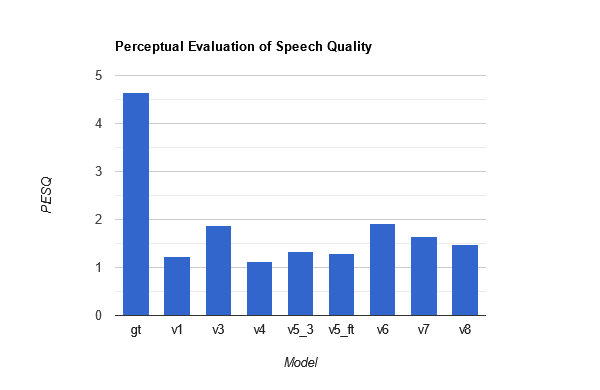
\includegraphics[width=\textwidth]{evaluation/graphs/PESQ.png}
    \caption{Perceptual Evaluation of Speech Quality results per model}
    \label{fig:pesq_results}
\end{figure}

Figure \ref{fig:pesq_results} shows the results of the PESQ evaluation on each
model. The first bar with a value of 4.64 is the reference value with a perfect
score. The graph clearly shows that the models we evaluated do not come close to
what is considered an excellent result in PESQ. The best models according to
PESQ are \emph{v3} and \emph{v6}.

\subsubsection*{F0 Root mean square error (F0 RMSE)}
The F0 value of speech, often also referred to as pitch or fundamental
frequency, is measured in Hertz, and describes the rate of vibration of the
vocal folds. The range of F0 is usually between 50 Hz to 450 Hz. This evaluation
compares the extracted F0 values from the original sound files to the ones
generated with each model. With the resulting differences, the root mean square
error is calculated to be able to assign each model a single score value. When
comparing specific extracted values of sound files, it is usually needed to use
dynamic time warping (DTW) to match the corresponding values to each other. In
our case this was not needed, as we already aligned each file using DTW before.
The reference value when comparing the original sound files with themselves, is
0.0 as there is no difference between them and therefore no error.

\subsubsection*{F0 RMSE results}
\begin{figure}[hbtp]
    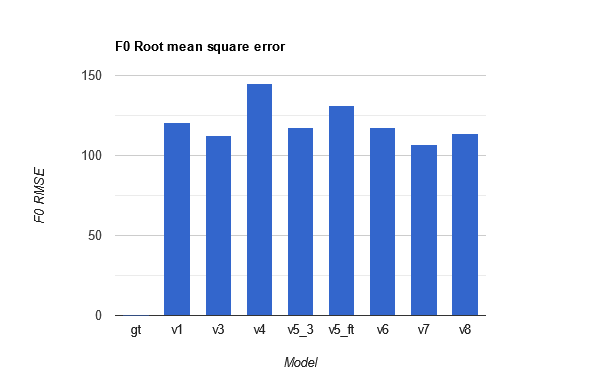
\includegraphics[width=\textwidth]{evaluation/graphs/F0RMSE.png}
    \caption{Fundamental frequency root mean square error}
    \label{fig:f0rmse_results}
\end{figure}

The chart in figure \ref{fig:f0rmse_results} shows the root mean square error of
the fundamental frequency, sometimes also referred to as pitch, for each model
we used. The shown reference value of 0.0 for \emph{gt} is a perfect value and
therefore usually not achieved in real calculations.

\subsubsection*{Speech-to-Noise ratio (SNR)}
The Speech-to-Noise ratio (SNR) compares the ratio of speech in a sound file, to
the amount of background noise. The formula used in this evaluation is \\
\[
    SNR = 10*log_{10} (\frac{RMSE(signal)}{RMSE(noise)})
\]
as formulated in \cite{ji2020comprehensivesurveydeepmusic}. The SNR is equal to 10 times the 10th log of the RMSE of
the original file (signal) divided by the RMSE of the generated file (noise). It
is usually measured in decibels (dB). The reference value for a perfect ratio is
0.0 as shown by comparing the original sound files to themselves.

\subsubsection*{SNR results}
\begin{figure}[hbtp]
    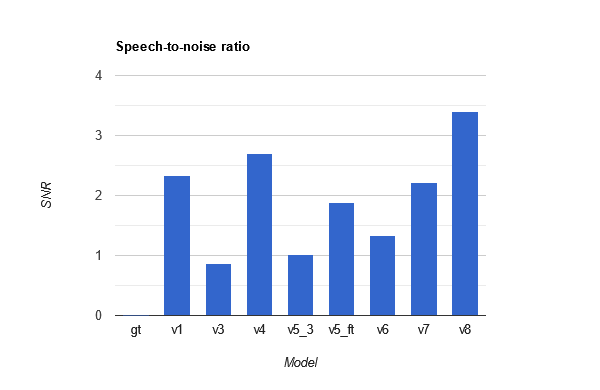
\includegraphics[width=\textwidth]{evaluation/graphs/SNR.png}
    \caption{Speech-to-noise ratio}
    \label{fig:snr}
\end{figure}

While SNR usually refers to Signal-to-noise ratio, and describes the ratio of
the wanted signal, and background noise, in our case it refers to
Speech-to-noise ratio. It describes the ratio of speech to background noise.
Figure \ref{fig:snr} shows the reference value of 0.0 for the ground truth and
the respective values for the used models. In this case model \emph{v3} is the
best one according to the SNR.

%==============================================
%============= Mixing and Mastering ============
%==============================================
\section{Mixing and Mastering}



%==============================================
%================ Conclusion ===================
%==============================================
\section{Conclusion}

Conclusion
The goal of our project was to develop an SVS model that could replicate the unique voice of Chester Bennington. Our approach focused not just on the training itself, but on creating a comprehensive pipeline that would allow others to have a guide that covers everything from data processing, data augmentation, training, evaluation and post-processing of the data to be able to use DiffSinger with their own data. So our intention is not just to create a replica of Chester's voice, but to provide an understandable guide to creating a DiffSinger model.

After creating our dataset with the unprocessed audio, we began pre-processing, an important step that determines the quality of our model. The first step was to extract the vocals to ensure that the model was only trained on relevant vocal data. This was followed by the segmentation and alignment of the data, as well as the creation of ds-files, which are needed for the use of DiffSinger.

This first preprocessing was followed by a second, which focussed on improving the quality of the data. For this purpose, some songs were edited manually so that disturbing noises and inappropriate sequences (e.g. wrong singer) were cut out. Some scripts also filtered out faulty segments. The alignment and ds-file creation steps were then repeated.

For the data augmentation process, we explored both DiffSinger's built-in augmentation functions and manual augmentation methods. While the built-in methods included pitch shifting and time stretching, we also applied pitch shifting, volume adjustment, noise reduction and velocity change to simulate real-world variations in vocal performance.


Setting up the training presented us with some challenges in terms of configuring the environment, setting up the hardware and dealing with outdated documentation. We initially tried to use Docker, but ran into issues with the module locations, so we decided to switch to a more reliable Anaconda environment. Once we had configured our system, we trained our models on the LST servers at Saarland University using HTCondor to schedule training jobs. The training progress was monitored with TensorBoard.

We trained different models experimenting with different parameters such as the size of the dataset, different quality of the dataset, the use of data augmentation, different vocoders and different learning rate and fine-tuning settings.


Despite the many different experiments, the results of the models are relatively comparable. Some segments are processed well by (almost) all models,however, the output of other segments is inadequate, as the voice sounds distorted and rough or other background noises appear to be involved. In many segments, the phonemes or phoneme boundaries also appear to be incorrect. To quantify model performance, we applied two types of evaluation: predicted Mean Opinion Score (MOS) using SingMOS and a mel-spectrogram histogram comparison. The variance+vocoder model consistently outperformed others across both evaluation types, with MOS scores approaching the ground truth and strong spectral similarity to real vocals. However, even this best-performing model could not fully replicate the expressive detail and clarity of the original vocals, often struggling with distorted phonemes, rough transitions, or alignment errors. 

A probable issue could be the automatic alignment. To address this problem, aligning the data manually would almost certainly lead to a better model as many boundaries are inadequate. However, this step requires a non-negligible amount of time, offering potential for future research. There can also be made improvements within the data augmentation as the project has highlighted the importance of careful and balanced augmentation to avoid degrading the model’s performance.

The main contribution of this project is the creation of a comprehensive guide for setting up and training a DiffSinger model, from data pre-processing to fine-tuning the model and post-processing. By documenting each stage of the process, we provide a valuable resource for others who wish to emulate or improve upon our work in speech synthesis. This guide serves as a step-by-step reference for anyone interested in training a speech synthesis model with DiffSinger, covering not only technical details, but also the challenges we encountered and how they were overcome.


To summarise, this project has provided valuable insights into the use of DiffSinger for voice replication, particularly in terms of data pre-processing, augmentation, model setup and post-processing. Our project also highlights the shortcomings of the results, which are mainly due to poor alignment and insufficiently high-quality data (e.g. an insufficient number of acapellas).  Therefore, further refinements are needed to fully capture the nuances of a unique voice like Chester Bennington's. Nonetheless, our efforts have established a solid foundation for future research and development in the field of voice synthesis, with the guidelines presented here providing a robust framework upon which others can build.

%==============================================
%================ Sources ===================
%==============================================

\bibliographystyle{plain}  % This style sorts references alphabetically
\bibliography{references}  % This will load your references.bib file



\end{document}
